\subsection{Results}

During the course of the diary study, we collected $868$ search entries with an average of 27 entries per person. 9\% of searches (33 out of 868) failed, not providing users with the information they sought. Participants performed an average of $1.2$ searches ($median=1, min =1, max=5$) and followed $2.5$ links ($median=2, min=0, max=39$) to find their information. Participants rated search difficulty at an average of $1.9$ ($median=2,  \sigma=1$). 

We categorized searches by type and difficulty. Searches were imprecise or general (browsing) when they employed more than one query or three or more links clicked in results. Otherwise, the searches were precise (fact finding). Searches were too hard when they failed, users rated them difficult ($4$ or $5$ on the scale), or they required more than $2$ minutes of searching. Otherwise, searches were easy. 

Using these two categories, were were able to bin the searches into four combined groups. 49 \% of the queries were precise and easy, 7 \% were precise and difficult, 20 \% were imprecise or general and easy, and 24 \% were imprecise or general and difficult. Table 1 shows various corresponding examples.
% We may want to add few of these comments: "could not come with the right descriptors for the mirror to find the one I had seen in the store." "had to navigate lots of links to find something useful" "had a hard time finding the right video of the musician as I didn't remember his name" "could not come up with the right search terms to find a book by a particular author and did not remember the author"

Although search was usually successful, it was difficult about a third of the time (31\%), especially when search was more imprecise or general. In fact these searches formed the large majority of the difficulties users were having. Further, roughly one third of imprecise and general searches sought information from datasets organized by entity relationships, such as movies and crews (\url{www.imdb.com}) or recipe ingredients and dishes (\url{allrecipes.com}). (This number may be significantly larger, because many participants only recorded their search tool, not the information they sought).

In sum, we believe the large majority of problem searches could have benefited from a tool that helped users navigate through the information neighborhoods typical of imprecise and general search, and that a good starting point for such a tool would be exploiting the structure available in many datasets. 

% Vidya: I don't think these two paras are relevant to this paper. Ben: agreed.

%The average time taken to record a search activity was $131.6$ seconds ($median=120, max=1200$). 
%People use applications more than websites for certain activities. On an average, 18.5\% (160 out of 868) of the searches were using applications than web portals. The most popular category searched using an application was \emph{shopping} (47\%). Surprisingly, participants frequently knew the exact keyword to put in as a search phrase. People use mobile apps for regular, standard search activities (i.e. weather, shopping, location, names, exchange rate, bus route, definition). For less frequent, more complicated searches, they will try it on a web portal but easily give up because of the screen size restriction and choose another method (i.e. go to their desktop, ask friends).

%
%We looked for duplicate themes from collected diary entries and did not start with a set of fixed categories. We adopted most of the categories from \cite{chi2008} and added new categories such as `\emph{how-to}', `\emph{unit conversion}', `\emph{definition}', and `\emph{name}'. There are 17 categories based on the diary entries.
%The \emph{how-to} category includes information about practical advice and detailed instruction of an activity. The \emph{unit conversion} includes kilometer to miles conversion, fahrenheit to celsius, and exchange rate. The \emph{definition} includes any need of terminology definition and detailed explanation. The \emph{name} includes search of a certain person or movie title. The largest category of collected entries was \emph{trivia} (51\%). They are the random thoughts from the participants such as ``story of shutter island". The second highest was \emph{shopping} (13\%), followed by \emph{point of interest} (10\%) and \emph{definition} (6\%).



%Vidya: I think this figure is hard to understand and looks too complicated. Ben: agreed.
%Figure \ref{fig:searchtype} categorizes search type of diary entries by success/failure, easy/difficult, open/specific queries, and hit or miss. Overall, the large blue section shows that people are mostly successful in finding information with their mobile device (though they may never attempt many challenging searches). About a third of searches are still difficult, and over half of difficult searches are open. 
%
%
%\begin{figure}[ht]
%\centering
%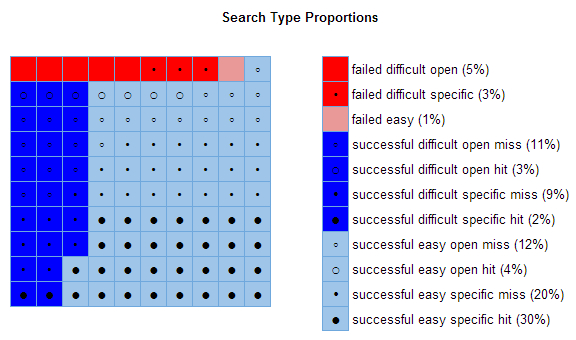
\includegraphics[width=3in]{images/searchtype}
%\caption{Search type by success/failure, easy/difficult, open/specific, and hit/miss. Blue: success, red: failure, saturated color: easy, bright color: difficult, empty dot: open, filled dot: specific, smaller dot: miss, bigger dot: hit}
%\label{fig:searchtype}
%\end{figure}




